\section{Systemmodell}

\subsection{Systemdiagramm}

\begin{figure}[H]
    \centering
    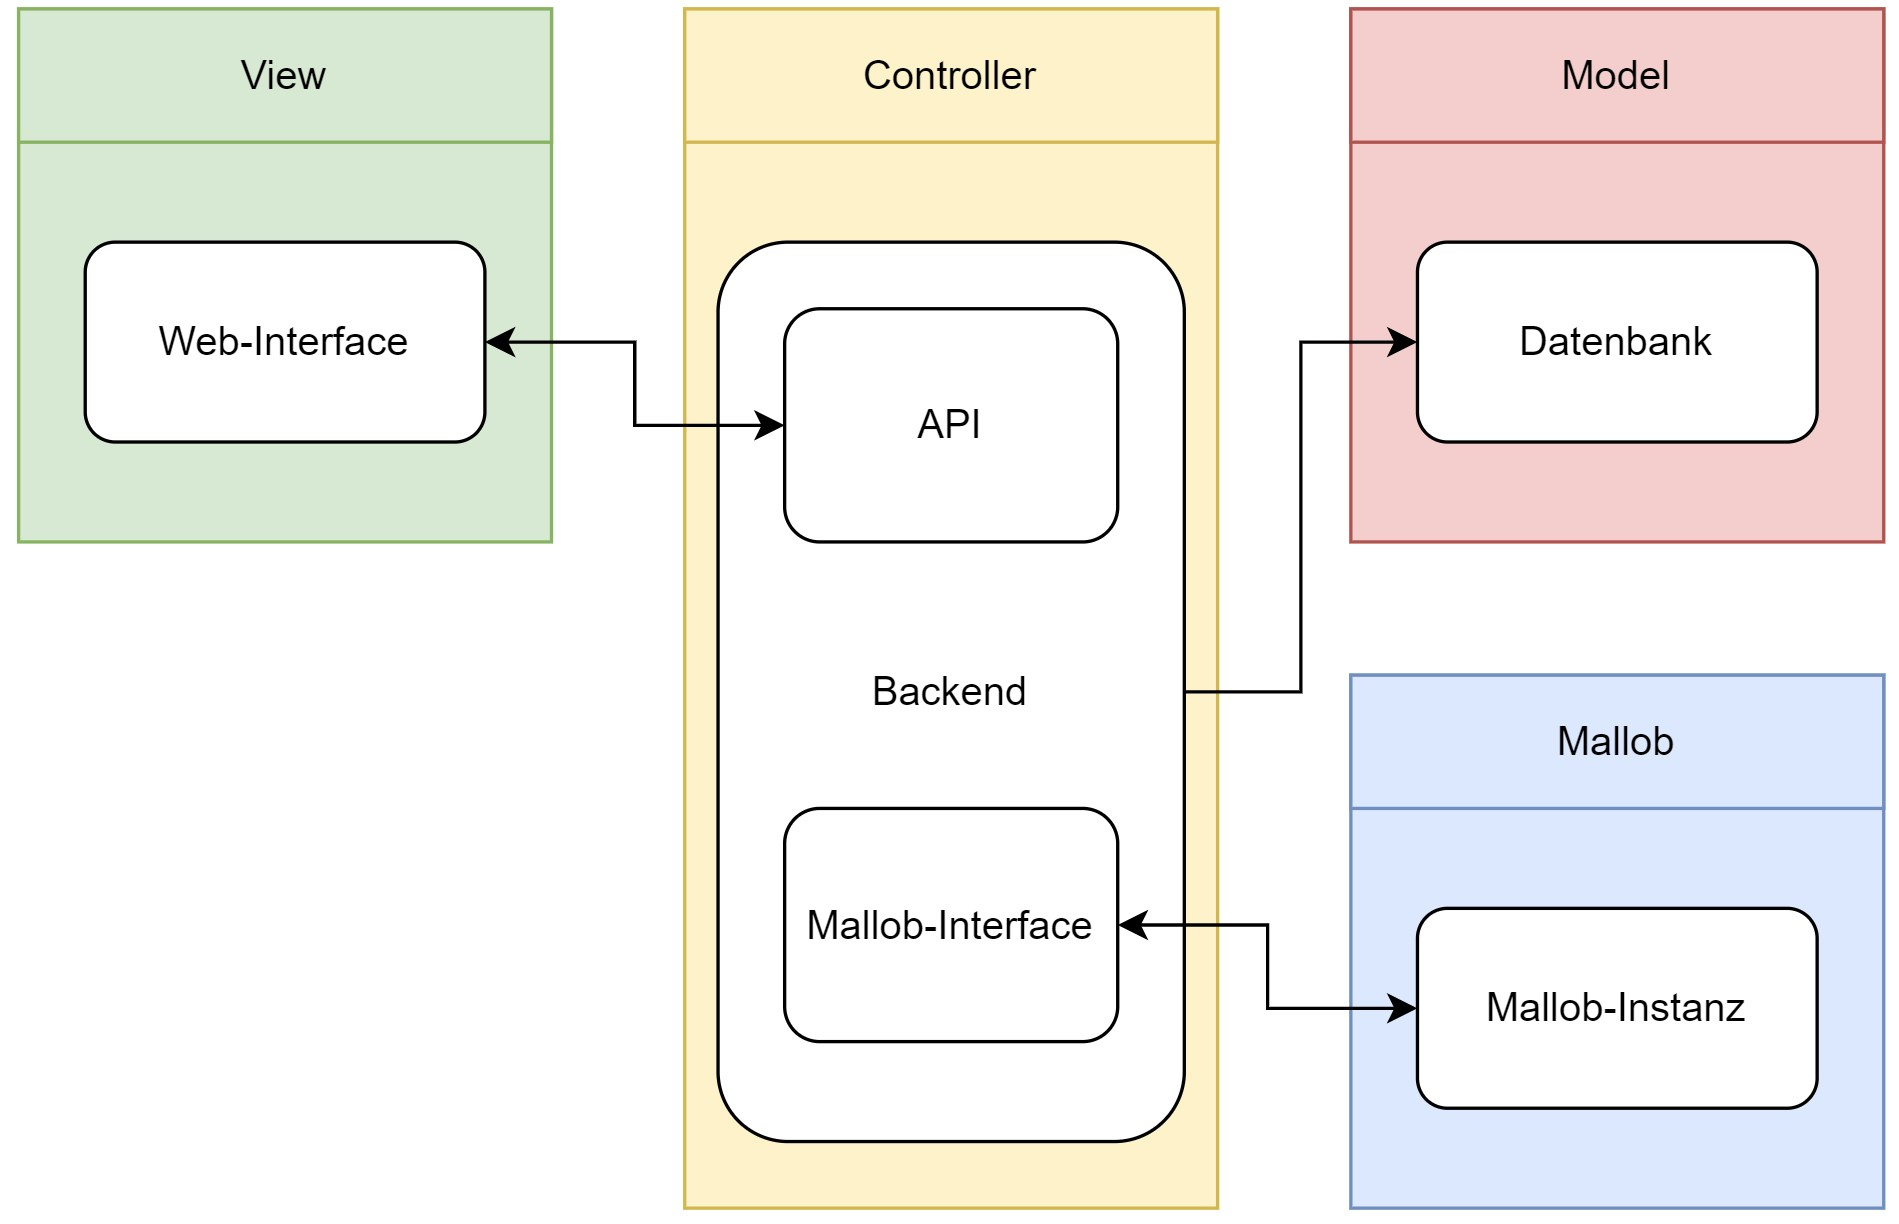
\includegraphics[width=\textwidth]{images-interface/Diagramme/Systemdiagramm3.jpg} \\
    \caption{\gls{Model-View-Controller}}
\end{figure}
Das System kann semantisch in 3 Komponenten gegliedert werden; View, Controller sowie Model. \\
Die Aufgabe des \textbf{Views}, bzw. des Web-Interfaces ist es dabei eine interaktive, grafische Benutzeroberfläche für die Interaktion mit Mallob bereitzustellen. \\
Der \textbf{Controller}, bzw. \gls{API} sowie Backend (Anfragen gehen über \gls{API} an das Backend) sind für die Kommunikation zwischen \gls{Datenbank}, Mallob und Web-Interface, bzw. \gls{Nutzer} zuständig. Das Mallob-Interface ist im Backend implementiert und für die Kommunikation zwischen der Backend-Logik und einer laufenden Mallob-Instanz zuständig.\\
Im \textbf{Model} hält eine \gls{Datenbank} die \hyperref[PD]{Daten des Systems} und Mallob ist Mallob. \\
\textbf{Extern} liegt die laufende Mallob-Instanz. Mallob ist nicht Teil unseres Systems. Unser System kommuniziert lediglich mit Mallob.

\pagebreak

\subsection{Anwendungsfalldiagramme}

\begin{figure}[H]
    \centering    
    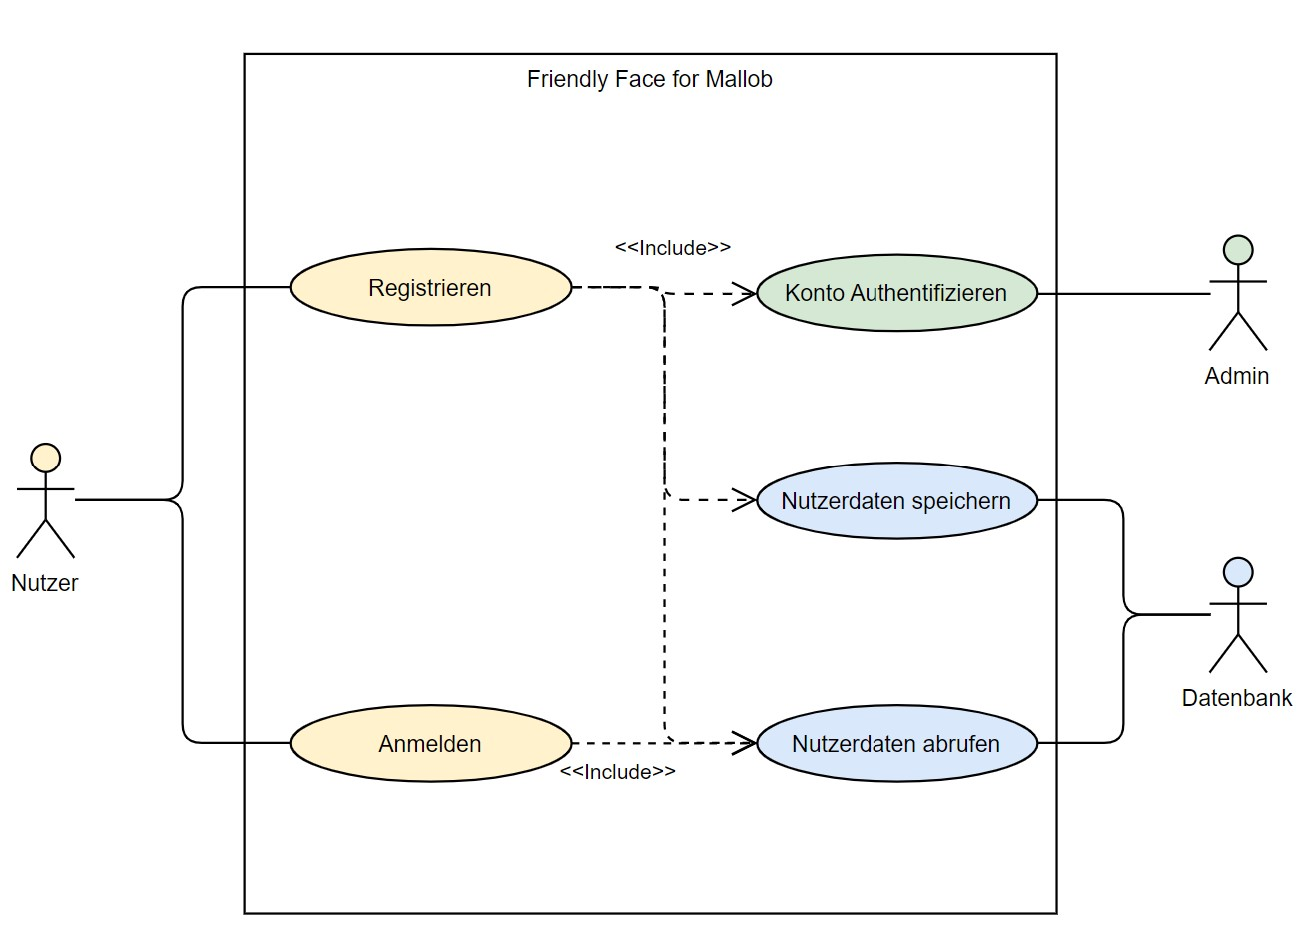
\includegraphics[width=\textwidth]{images-interface/Diagramme/Login_register_3_screenshot.jpg} 
    \caption{Registrierung von \gls{Nutzer}n}
\end{figure}


Registriert sich ein \gls{Nutzer}, so wird seine Registrierunganfrage von einem \gls{Administrator} verifiziert. Die \gls{Datenbank} speichert die \hyperref[PD:Nutzerdaten]{Nutzerdaten}.\\
Möchte sich ein registrierter \gls{Nutzer} im Web-Interface anmelden, so werden die Nutzerdaten aus der \gls{Datenbank} geholt und mit den eingegebenen Daten verglichen. \\
Stellt ein registrierter \gls{Nutzer} eine Anfrage über \gls{API} mit seinem \gls{Token}, wird auch hier der \gls{Token} aus der \gls{Datenbank} geholt und verglichen.
\begin{figure}[H]
    \centering
    \includegraphics[width=\textwidth]{images-interface/Diagramme/Request_authntification_screenshot.jpg}
    \caption{Authentifizierung von \gls{API}-Anfragen}
\end{figure}
Jede Anfrage an die \gls{API} muss authentifiziert werden. Dies geschieht, indem der \gls{Token}, der mit der Anfrage geschickt wurde, mit dem in der \gls{Datenbank} gespeichertem \gls{Token} abgeglichen wird. Wurde eine Anfrage verifiziert, also sichergestellt, das der \gls{Nutzer} diese auch ausführen darf, so wird sie weiterverarbeitet.\\
Jede Anfrage an die \gls{API} wird für eine gewisse Zeit gespeichert, um sie später noch einmal referenzieren oder einsehen zu können.

\pagebreak

%https://www.overleaf.com/project
\begin{figure}[H]
    \centering
    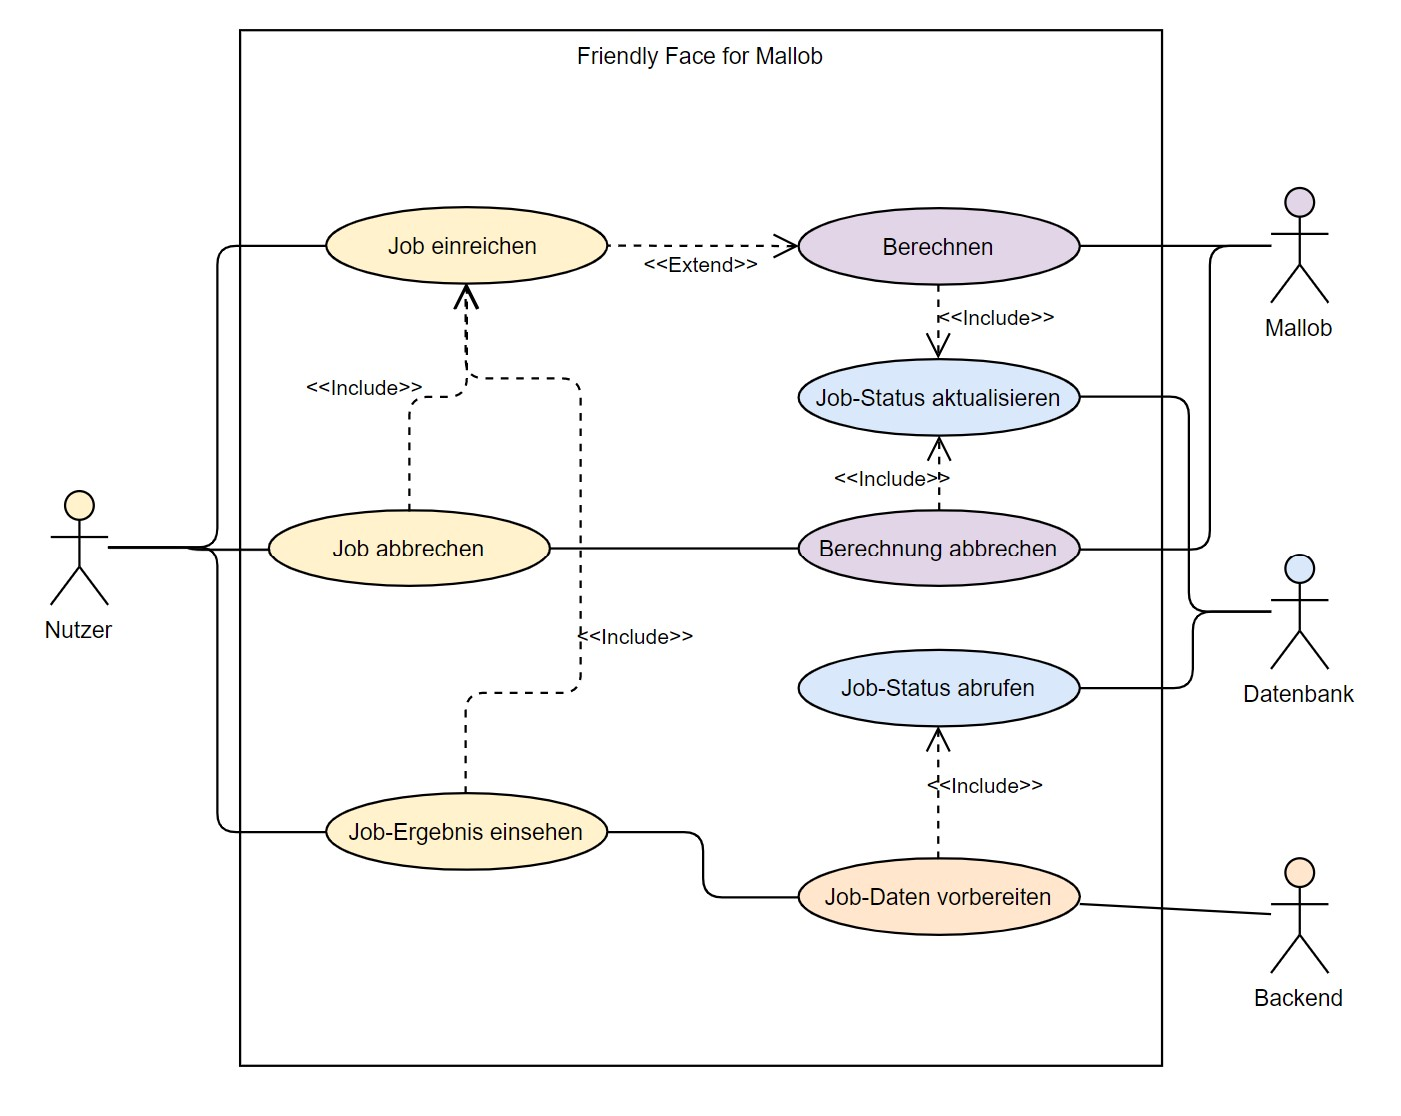
\includegraphics[width=\textwidth]{images-interface/Diagramme/Submit-abort-view-screenshot.jpg}
    \caption{Einreichen, Abbrechen und Einsehen von Jobs}
\end{figure}

Reicht ein \gls{Nutzer} ein Job ein, so wird dieser (je nach Konfiguration) von Mallob bearbeitet. Mallob gibt dabei Rückmeldung über den Job-Status, also entweder das Ergebnis des Jobs, oder ob ein Fehler aufgetreten ist. Dieser Status wird in der \gls{Datenbank} gespeichert. \\
Ein \gls{Nutzer} kann die Bearbeitung eines Jobs, der gerade von Mallob berechnet wird, abbrechen. Die berechneten Zwischenergebnisse werden dann gespeichert und können später abgerufen werden. \\
Möchte ein \gls{Nutzer} einen Job einsehen, so ist es wichtig das dieser bereits eingereicht wurde. Um ein Job einsehen zu können werden zunächst die angeforderten Job-Daten aus der \gls{Datenbank} geholt und dann vorbereitet an den \gls{Nutzer} geschickt.



%\begin{center}
%    \includegraphics[scale=0.6]{images-interface/Request_authntification_screenshot.jpg} \\
%    Anwendungsfalldiagramm 2: Authentifizierung von \gls{API}-Requests
%\end{center}


\begin{figure}[H]
    \centering
    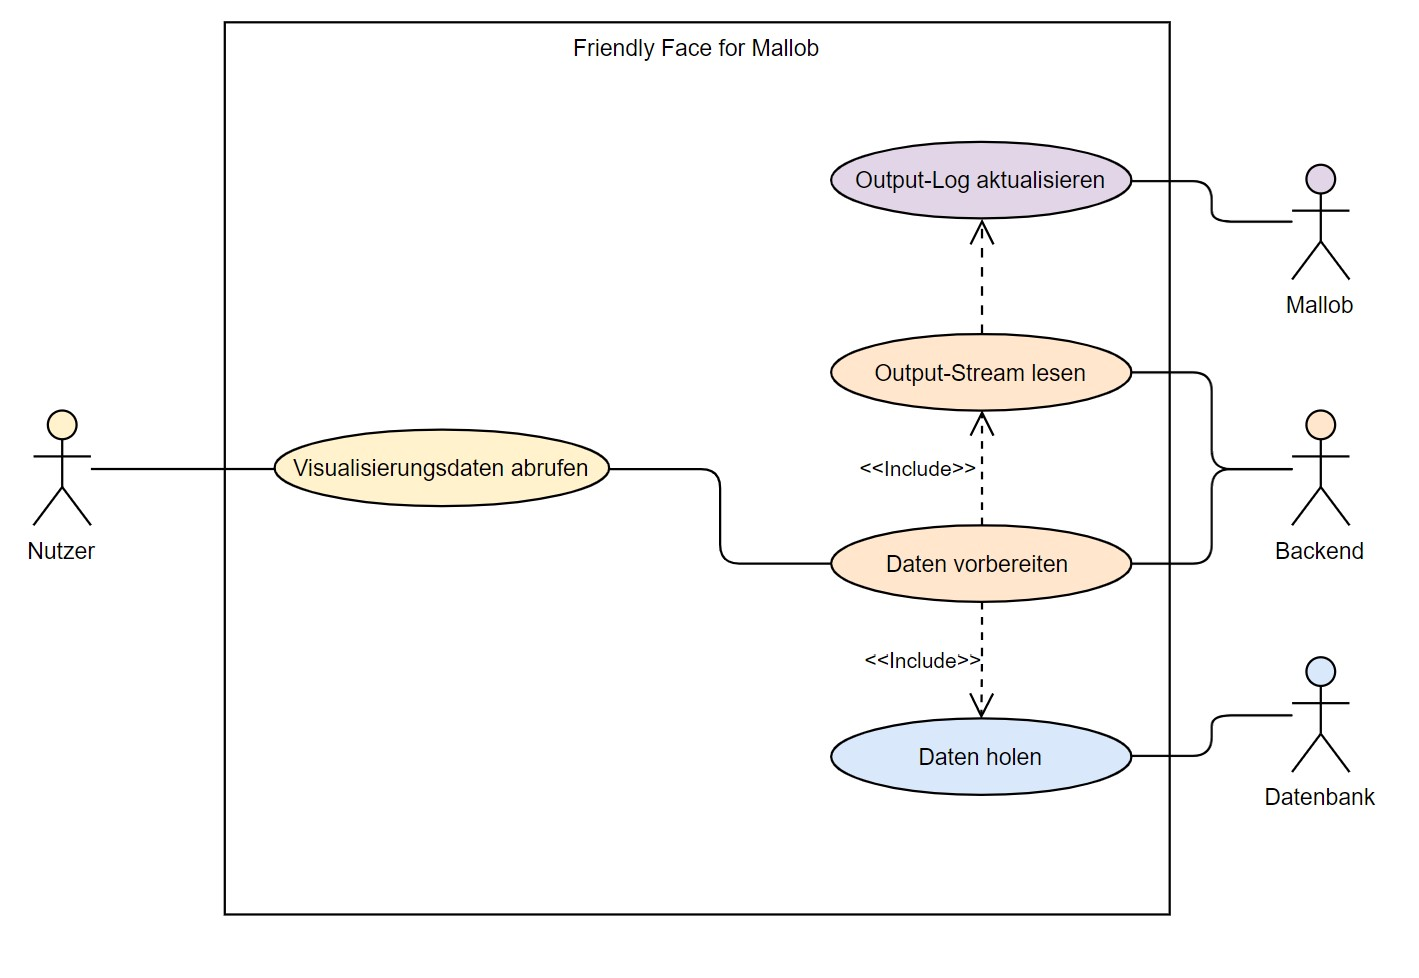
\includegraphics[width=\textwidth]{images-interface/Diagramme/visualisierungsdaten_anwendungsfaelle.jpg}
    \caption{Mallob-Visualisierungsdaten abrufen}
\end{figure}
Möchte ein \gls{Nutzer} Mallob-Visualisierungsdaten abrufen, so holt das System bereits vergangene Events aus der \gls{Datenbank} um hieraus die Visualisierung vorzubereiten. Des weiteren wird live der Output-\gls{Stream} der \gls{Log-Datei} von Mallob ausgelesen, um Echtzeit-Visualisierung für den \gls{Nutzer} anzubieten. 


\pagebreak

\subsection{Aktivitätsdiagramme}
\begin{figure}[H]
    \centering
    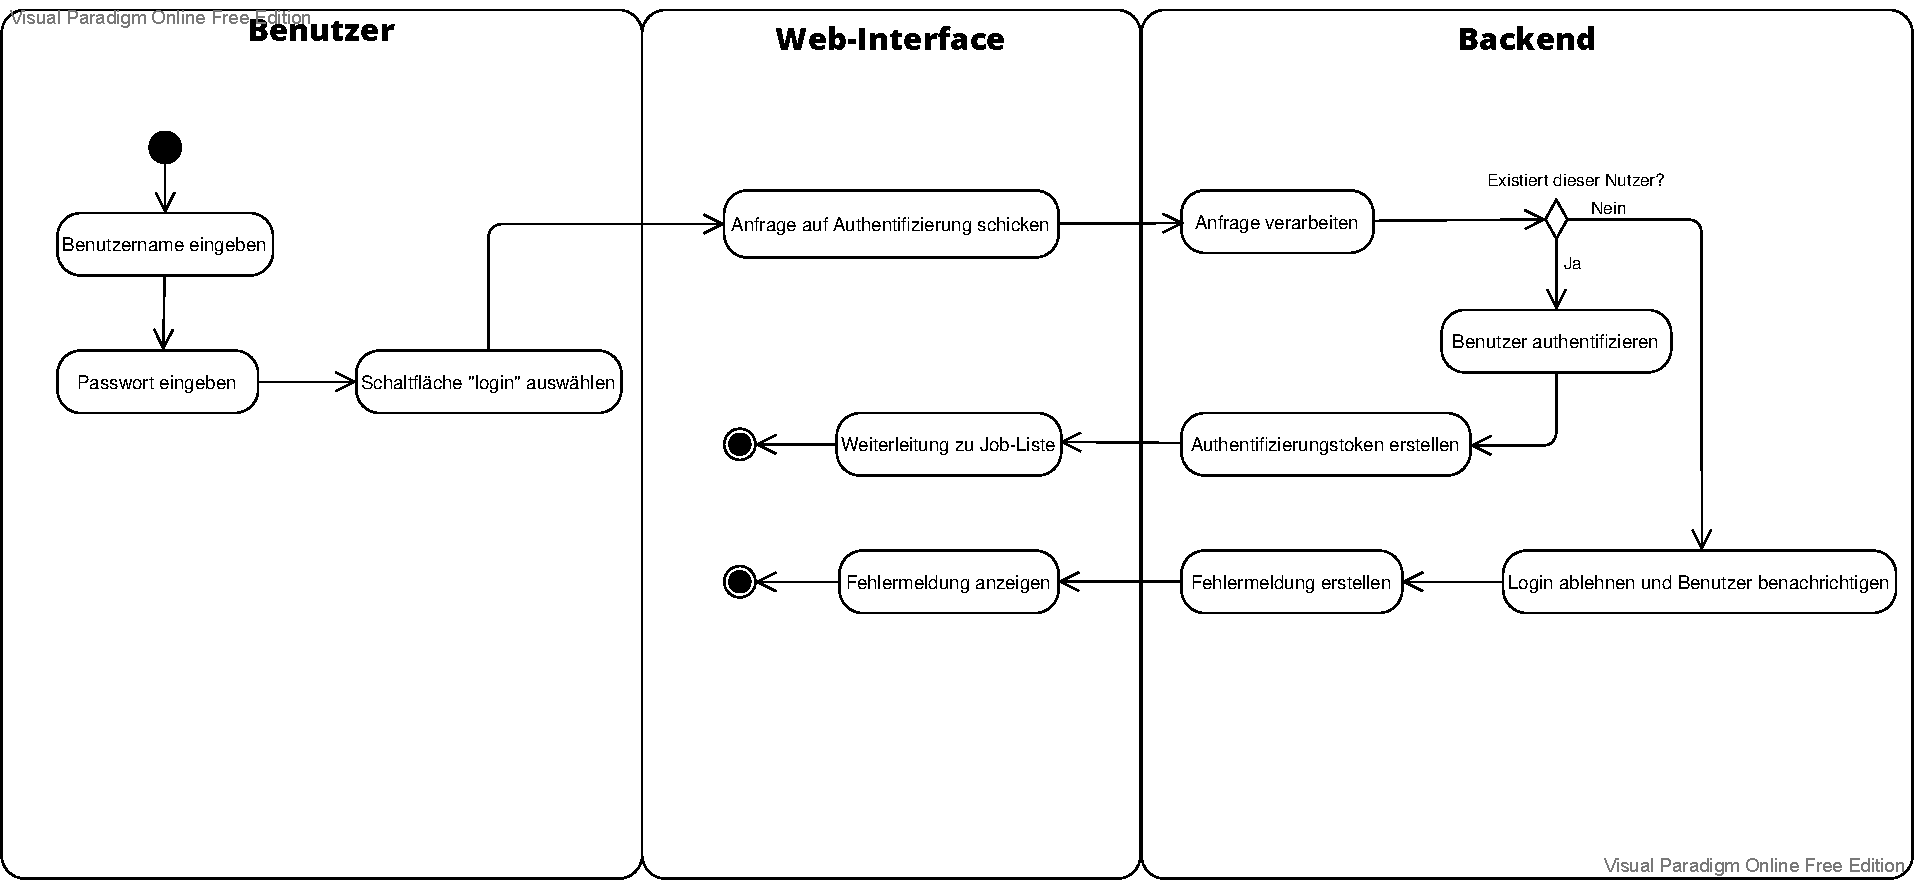
\includegraphics[width=\textwidth]{images-interface/Anmelden_Aktivitaetsdiagramm.pdf}
    \caption{Anmeldung im System über das Web-Interface}
    \label{fig:login_activity}
    
\end{figure}
Das Diagramm zeigt das folgende Situation: Ein \gls{Nutzer} besitzt im Moment kein authentifizierungs-\gls{Token} und muss sich anmelden, um die Funktionen der \gls{API}/Web-Interface zu benutzen. Zuerst gibt das \gls{Nutzer} über die Eingabe-Maske seinen Benutzername und Passwort und klickt auf die Schaltfläche "login", wobei das Web-Interface seine Anfrage an der \gls{API} zur Authentifizierung schickt. Das \gls{API} überprüft die Daten und hat zwei Möglichkeiten: Entweder existiert der \gls{Nutzer} mit dieser Kombination von Daten im System, wobei ihm ein authentifizierungs-\gls{Token} erstellt wird und das Web-Interface leitet ihn auf seine Job-Liste Seite weiter, oder es wird die Anmelde-Anfrage abgelehnt und eine Fehlermeldung vom Web-Interface an dem \gls{Nutzer} gezeigt.


\begin{figure}[H]
    \centering
    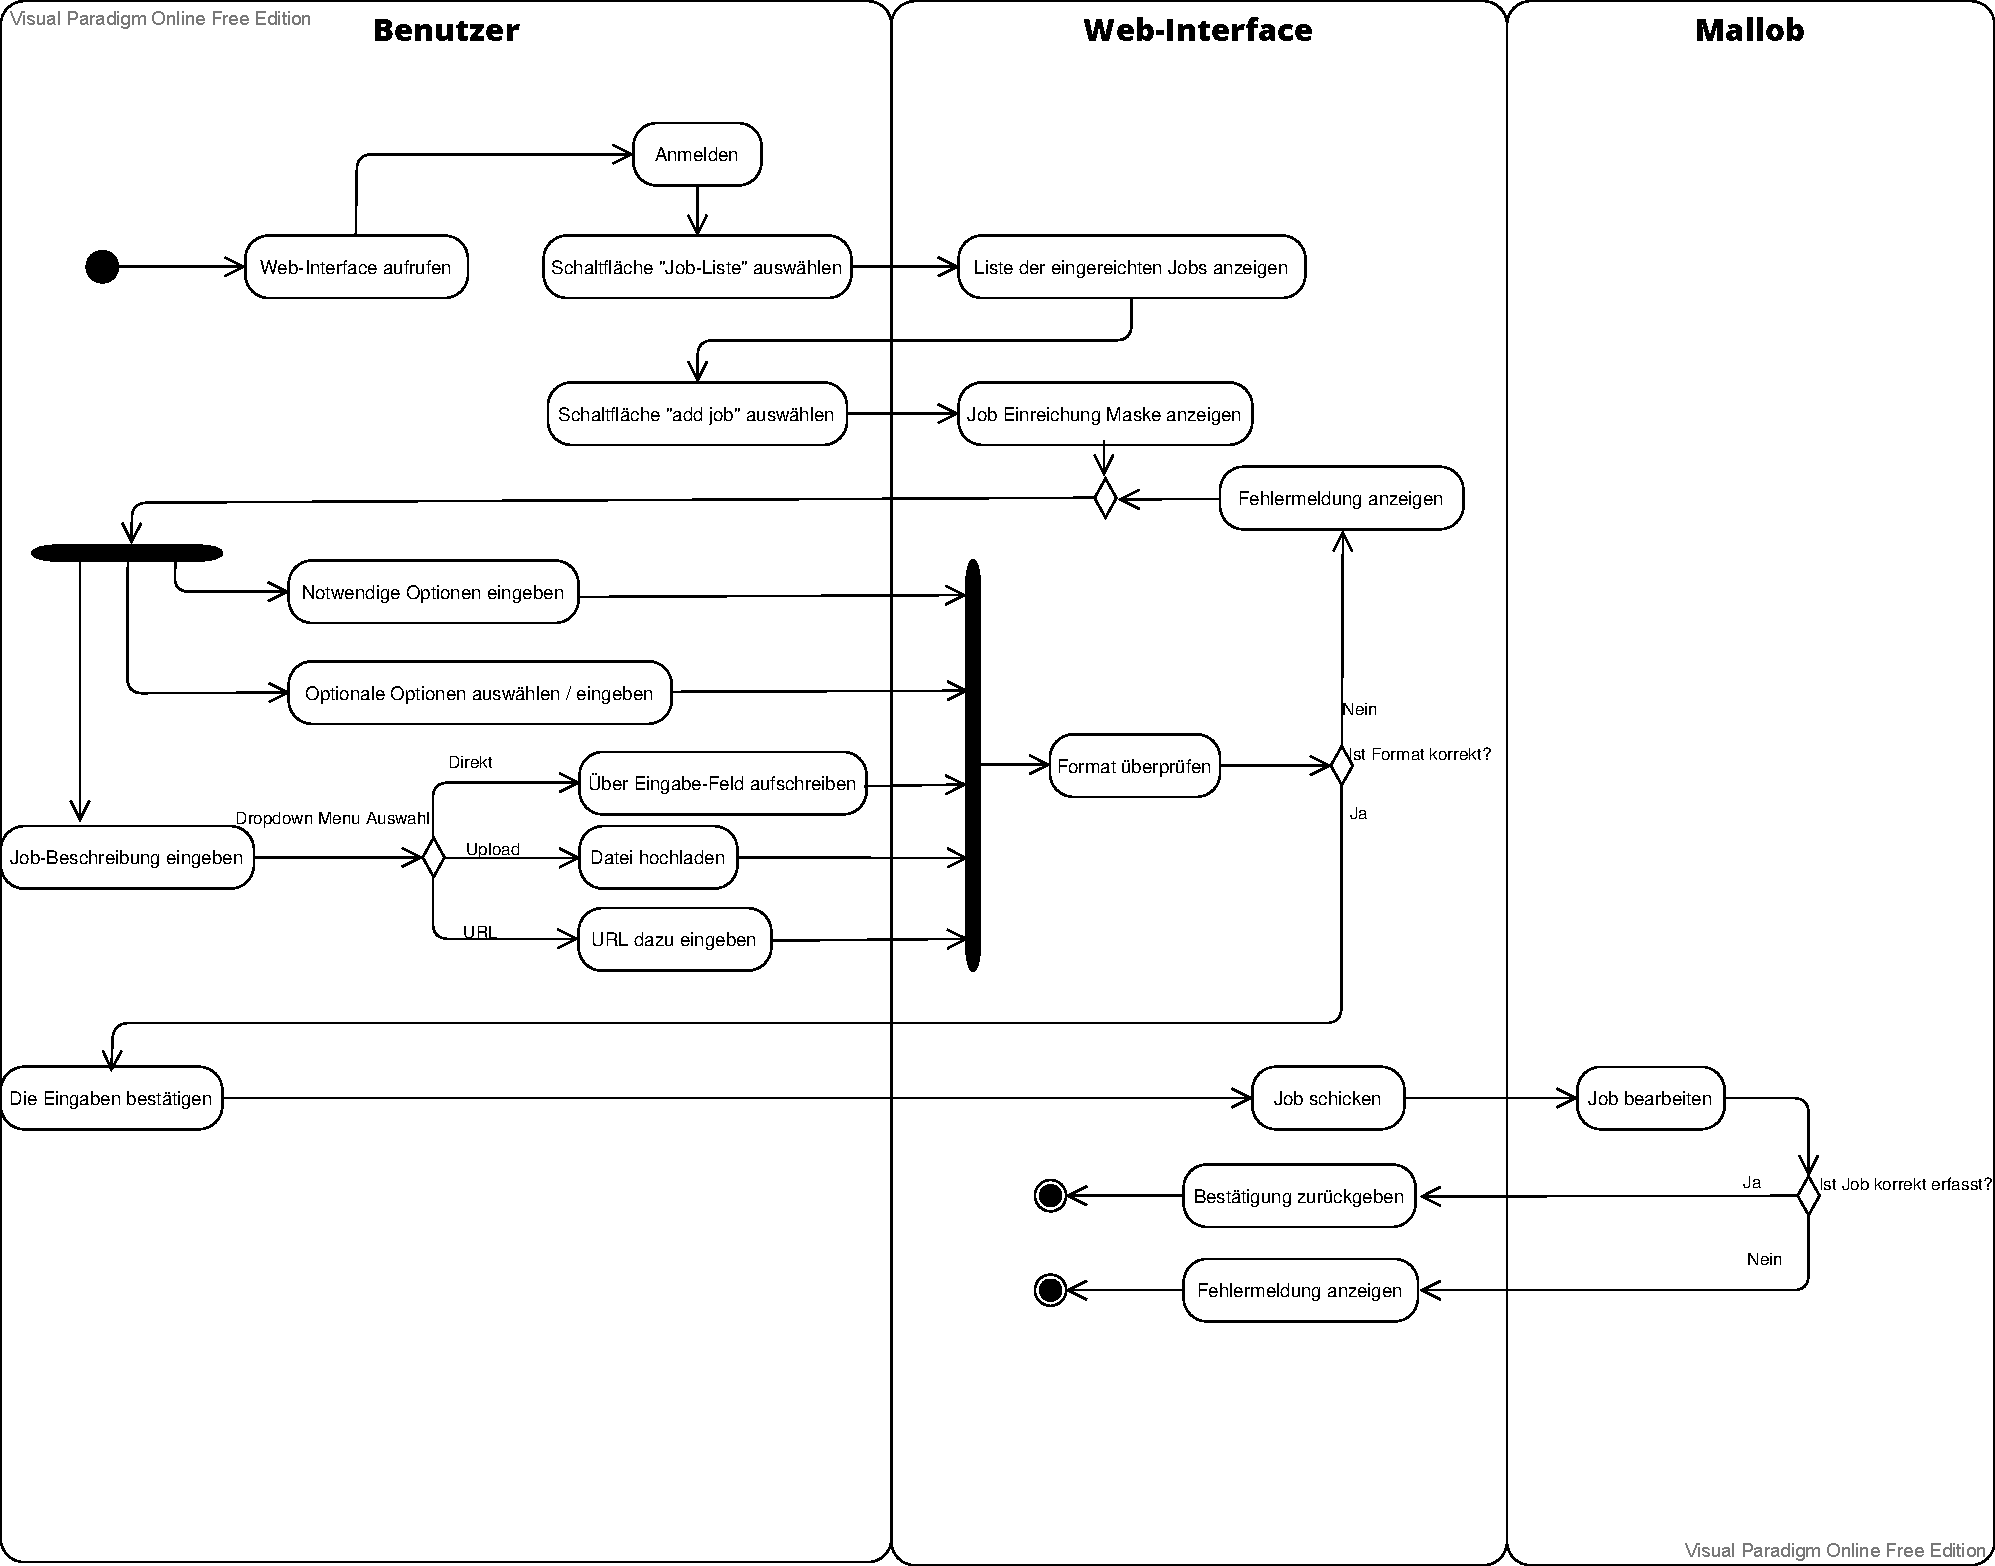
\includegraphics[width=\textwidth]{images-interface/Job_einreichen.pdf}
    \caption{Einreichen eines Jobs über das Web-Interface}
\end{figure}
Möchte ein \gls{Nutzer} Jobs einreichen, muss er angemeldet sein. Danach klickt er die Schaltfläche "Job-Liste" an, wobei eine Liste von eingereichten Jobs über das Web-Interface angezeigt wird. Dann wählt man die Schaltfläche "add-job" und ihn wird über das Web-Interface eine Eingabe-Maske angezeigt. Hier muss man die notwendigen Optionen eingeben, die optionale Optionen auswählen und die Job-Beschreibung auf eine der drei Weisen eingeben. Dabei wählt man von einem Drop-Down-Menu, ob man das direkt aufschreibt, mittels "upload" eine Datei damit hochladen oder ein URL dazu eingibt. Hier wird das Format der Eingaben vom Web-Interface überprüft. Falls das Format inkorrekt war, muss der \gls{Nutzer} die inkorrekte Eingabe verändern, andernfalls kann der \gls{Nutzer} die Eingaben bestätigen, was seine Job über das Web-Interface zu Mallob schickt. Mallob überprüft den Job-Inhalt und falls ein Fehler aufgetreten ist, wird diese vom Web-Interface angezeigt. Falls das Job vom \gls{Nutzer} korrekt erfasst worden war, wird eine Bestätigung zur Job-Bearbeitung/Lösung vom Web-Interface zurückgegeben.

\begin{figure}[H]
    \centering
    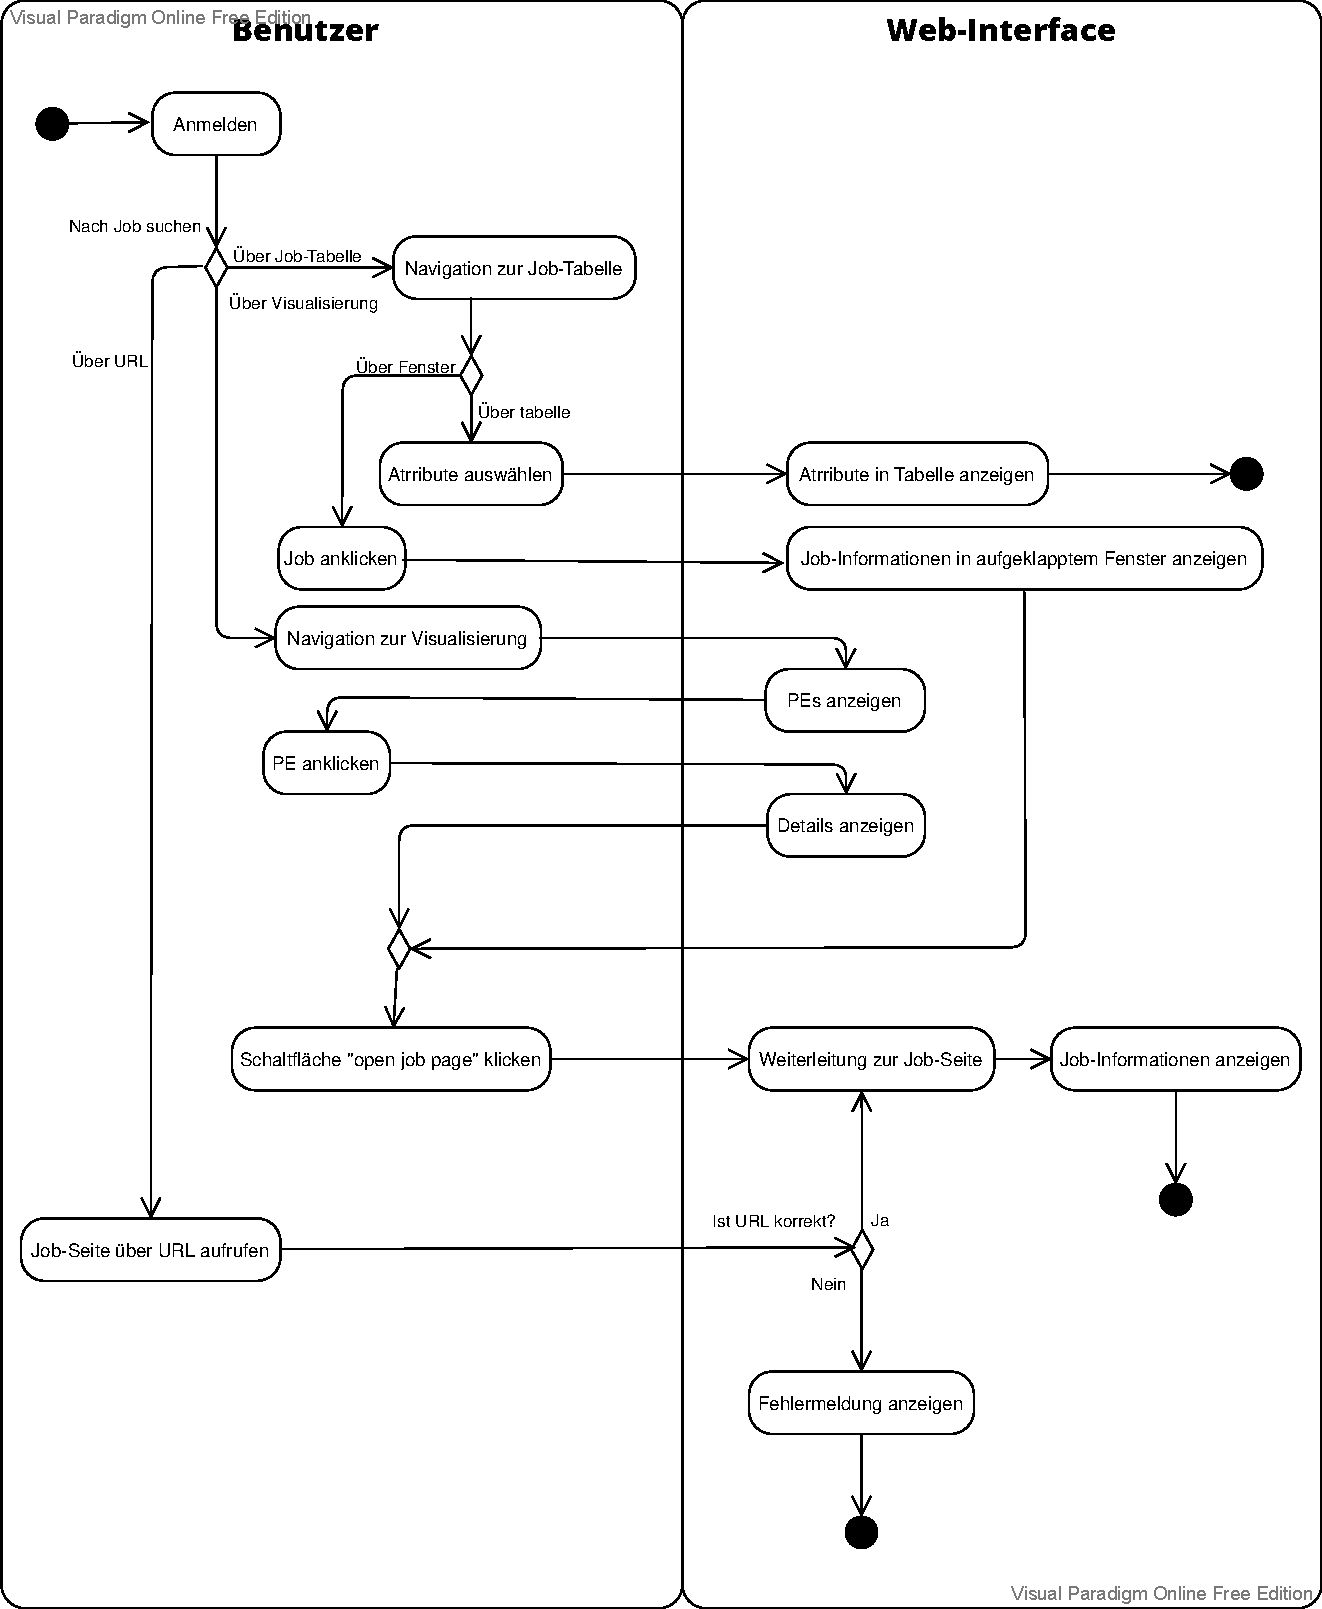
\includegraphics[width=\textwidth]{images-interface/get_infos.pdf}
    \caption{Einsehen von Job-Informationen}
\end{figure}
Hier werden die verschiedene Wege zum Einsehen der Job-Informationen angezeigt. Zuerst muss immer ein \gls{Nutzer} dafür angemeldet sein. Dann hat er 3 Möglichkeiten: 

1. Eine URL im Browser eingeben und die Job-Seite aufrufen. Falls die URL korrekt war, wird er zur Job-Seite weitergeleitet, wo ihm die Job-Informationen gezeigt werden. Falls die URL inkorrekt war, wird eine Fehlermeldung angezeigt.

2. Der \gls{Nutzer} klickt die Visualisierung Schaltfläche an, wobei das Web-Interface ihn die PEs zu seinem Jobs anzeigt. Der \gls{Nutzer} klickt auf eine von dieser und ihn werden Details dazu angezeigt. Dann klickt er die Schaltfläche "open job page", was ihn über das Web-Interface zur Job-Seite weiterleitet und da die Job-Informationen anzeigt.

3. Der \gls{Nutzer} navigiert sich zu der Job-Tabelle, die seine Jobs eingereichte enthält. Hier kann er entweder eine Attribute aus den Drop-Down-Menu auswählen, wobei ihn über das Web-Interface der ausgewählte Attribut zu alle Jobs angezeigt wird, oder eine der angezeigten Jobs anklicken und Job-Informationen in einen aufgeklapptem Fenster einsehen. Dabei kann man wieder die Schaltfläche "open job page" anklicken, was ihn über das Web-Interface zur Job-Seite weiterleitet und da die Job-Informationen anzeigt.
